\documentclass[a4paper, 11pt, parskip=half]{scrartcl}

\usepackage[english]{babel}
\usepackage[utf8]{inputenc}
\usepackage[T1]{fontenc}

\usepackage{listings}

\newcommand{\titleString}{Use of noisy constraints in Protein Structure
Prediction}
\newcommand{\groupName}{Methionine}

\usepackage[hidelinks,
            pdfauthor={\groupName},
            pdftitle={\titleString},
            pdfsubject={Computational Biology}]{hyperref}

\usepackage[utf8]{inputenc}
\usepackage[pdftex]{graphicx}
\usepackage{float}

\usepackage{authblk}

\title{\titleString}

\author{David Lassner}
\author{Moritz Neeb}
\affil{\groupName}

\graphicspath{{./plots/}}

\begin{document}

\maketitle

% According to https://www.isis.tu-berlin.de/2.0/mod/assign/view.php?id=84719:
% try to focus on the analysis of your results and the insights and future work you got from the projects.

%\section*{Abstract}
%TODO should we have an abstract? i dont think so. this is just a reminder to discuss it.

\section{Introduction}

\subsection{Background}

Ab initio protein structure prediction is hard.
%TODO reformulate previous sentence more scientific
To make it easier, ab initio protein structure prediction
can be enhanced by \emph{constraints}.
A constraints is an information about the proximity of residues in the native protein.
This information can be used to guide the prediction and possibly improve it.
Typically, a set of constraints is used together to guide the search.
These constraints can for example be a result of protein contact prediction,
which has to be run as a preliminary step.
%TODO can you say "has to be run"?
%TODO reference to Schneider/Brock 2014

\subsubsection*{Definitions}
\begin{description}
  \item[fulfilled constraints] are constraints that are within the range of $0$ and $8$ angstrom in a protein (decoy or native).
  \item[native constraints] are the fulfilled constraints in the native protein,
  i.e. those that are expected to guide the prediction towards the native structure.
\end{description}

\subsection{Technology Used}

The project's software consists of python and shell scripts that are used to
handle the constraint analysis and subset generation,
calls to Rosetta, overall analysis and plotting.

\subsection{Goal and Approach of this Project}
\label{sec:GoalApp}
%TODO split goal <-> approach??

In this project, noisy constraints were used.
That means, most of the constraints are misleading (i.e. not native),
as the contact prediction step is inaccurate.
%TODO reference to amount, e.g. 63 natives of 225 for 2h3jA
The challenge is to make use of the constraint set despite their noisiness.
The approach in this project basically contained three steps:
\begin{enumerate}

  %TODO conc. wording: group or subset? In the code, we said group,
  % but I think subset is better here.
  \item Constraint subsets
  were generated through a heuristic from which it was expected to get
  a high percentage of native constraints.

  \item The protein structure was predicted with these subsets of constraints as input.

  \item The information available (i.e. decoy scores and fulfilled constraints)
  was exploited to predict whether a subset
  contains native constraints or not.
\end{enumerate}

Two hypotheses were stated at the beginning and will be discussed in the following sections:
1) The native constraints produce better predictions.
2) The chance of a constraint to be native is higher if it is compatible with other constraints.

\subsubsection*{Subset Generation}
As it is computationally not feasible to run the structure prediction for every possible subset of the noisy constraints,
a heuristic has to be used, to get subsets that are promising.
This heuristic takes additional problem-specific information into account to shrink the search space to feasible cardinality.
The additional information can be mined from multiple sources, as e. g. 
\emph{a)} the distribution of the positions of input constraints on the sequence,
\emph{b)} priority by type of constraint source, for instance evolutionary based constraints over distances on decoys, or
\emph{c)} the secondary structure.
In this project, subsets were generated based on the information of secondary structure, whereas the successive steps of the analysis are independent of the heuristic and can be applied with any grouping. The subset generation based on the secondary structure works as follows:\\
Every constraint defines a desired spatial distance between two residues.
Given that the secondary structure of a sequence of residues is known, one can easily group the constraints based on the two secondary structures of the residues.
Thus, any subset can be identified by the two secondary structures, between which all constraints of this subsets are located.
%TODO example and figure
We assume, that the problem of identifying the secondary structure membership of a residue is already solvable with a high accuracy. 
If we consider the secondary structure of the protein to be rigid in a sense, that the energetic properties are minimal, it is unlikely, that the structure prediction improves by employment of constraints with both residues located in the same secondary structure. 
If a group is instead between two distinct rigid parts of the protein, the chance is higher, that Rosetta is able to enable the constraints during the folding process. 
In other words, the constraints are more likely to be compatible with each other. 
For that reason, we also leave out the constraint groups that are identified by at least one loop.

%\subsection{Penalty of Constraints}
%TODO Describe scoring and rescoring?

\section{Analysis and Results}
\begin{figure}
    \centering
    \begin{tabular}{ r || l | l }
      group & precision & recall \\
      \hline
      0 & 0         & 0 \\
      1 & 16.67     & 1.37 \\
      2 & 0         & 0 \\
      3 & 61.54     & 10.96 \\
      4 & 52.63     & 13.7 \\
      5 & 33.33     & 10.96 \\
      6 & 72.22     & 35.65 \\
    \end{tabular}
\caption{properties of the constraint groups of example protein 2krkA}
\label{fig:precisionRecall}
\end{figure}
In this section we will analyze the procedure presented in the \autoref{sec:GoalApp}. In analogy this section will contain three parts for each step in the procedure, namely the grouping, the rosetta run, and the choice of promising groups.
\subsection{Analysis of the grouping}
In \autoref{fig:precisionRecall} one can see, that some groups are meaningful, others are not. 
The precision and recall is computed based on the distances in the native structure and can not be used for the procedure. 
The table instead gives an idea of how well the grouping based on that simple heuristic works.
\subsection{Rosetta ab initio and scoring}
\begin{figure}
    \centering
    \begin{lstlisting}
    ./AbinitioRelax.linuxgccrelease
    
    -in:file:fasta input/2krkA/2krkA.fasta
    -in:file:frag3 input/2krkA/2krkA.200.3mers
    -in:file:frag9 input/2krkA/2krkA.200.9mers
    -in:file:native input/2krkA/2krkA.pdb
    
    -constraints:cst_file constraints.txt
    
    -out:nstruct 100
    -out:pdb
    
    -mute core.io.database
    -database /rosetta-3.5/rosetta_database/
    -abinitio:relax -relax:fast
    \end{lstlisting}
    \caption{Example call of Rosetta ab initio relax with which the experiment results were created}
    \label{fig:rosettaCall}
\end{figure}

For every group of constraints Rosetta ab initio is run with producing 100 decoys, as shown in \autoref{fig:rosettaCall}. In Rosetta, the constraints are enforced by adding a penalty function to the energy function for each constraint. The constraint type used is called \emph{bounded}, which corresponds to hydrogen bonds, that can occur in nature in a distance interval between close to zero and eight angstrom. Hence, the penalty function is set to have minima in that interval.

Since the energy function is modified by the constraints, it is not accurate to account the resulting scores. Instead to produce comparable results, the produced decoys are re-scored without a modified energy function.

\subsection{Choice of groups}
We chose different metrics to analyze the results of the Rosetta run. In principle the most common metrics are the Rosetta Energy Score and the GDT. %TODO: explain GDT
We added the \emph{ratio of enabled constraints} as another metric to compare the results. This metric corresponds to the idea of compatibility of a constraint set, because if Rosetta is able to enable all constraints given, it is proven, that the constraints are compatible, likewise if Rosetta fails to enable most of the constraints, it is a good indication for the set containing either not compatible, or not native constraints.

It turned out, that the energy score is not meaningful, instead there is very few difference between using \emph{a)} all native constraints, \emph{b)} a random subset set of all input constraints, or \emph{c)} no constraints at all. This can be seen in \autoref{fig:EnergyNativeBaselineRandom}\\
\begin{figure}
    \centering
    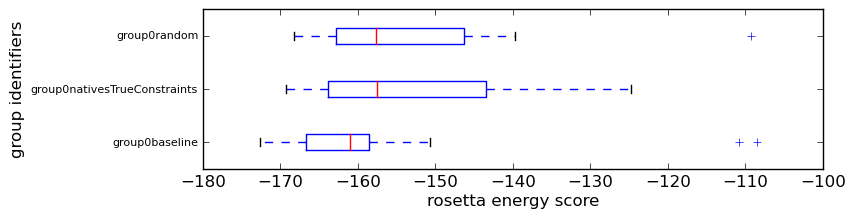
\includegraphics[width=0.7\textwidth]{EnergyNativeBaselineRandom.png}
    \caption{This image shows, that there is not a significant improvement of energy score between the decoys with native constraints and other, like the baseline (with no constraints) and a group with a random set of constraints picked from the input file. Note, that this scoring is done seperately from the ab initio and the energy function does not include constraint penalties.}
    \label{fig:EnergyNativeBaselineRandom}
\end{figure}
    
In contrast, the GDT shows significant difference comparing the decoys with all native constraints and other groups: The similarity to the native structure is very high when the native constraints are enforced (see \autoref{fig:GdtNativeBaselineRandom}). Unfortunately the GDT cannot be used for an iterative algorithm to predict the structure, because the native structure is unknown.\\
\begin{figure}
    \centering
    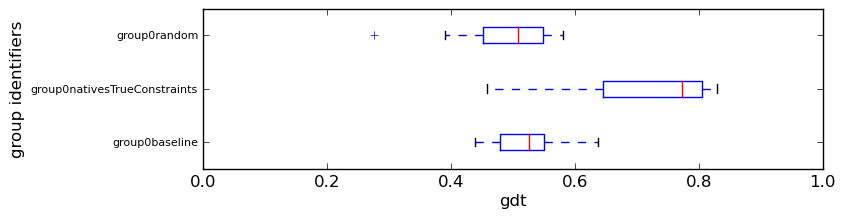
\includegraphics[width=0.7\textwidth]{GdtNativeBaselineRandom.png}
    \caption{This image shows the improvement of employing the native constraints. This demonstrates the importance of employing the correct constraints.}
    \label{fig:GdtNativeBaselineRandom}
\end{figure}

Finally, the metric of \emph{enabled constraints} shows a high variance over the groups and there is a meaningful relation between the values of precision / recall and the ratio of enabled constraints (\autoref{fig:enabledConstraints}). 
\begin{figure}
    \centering
    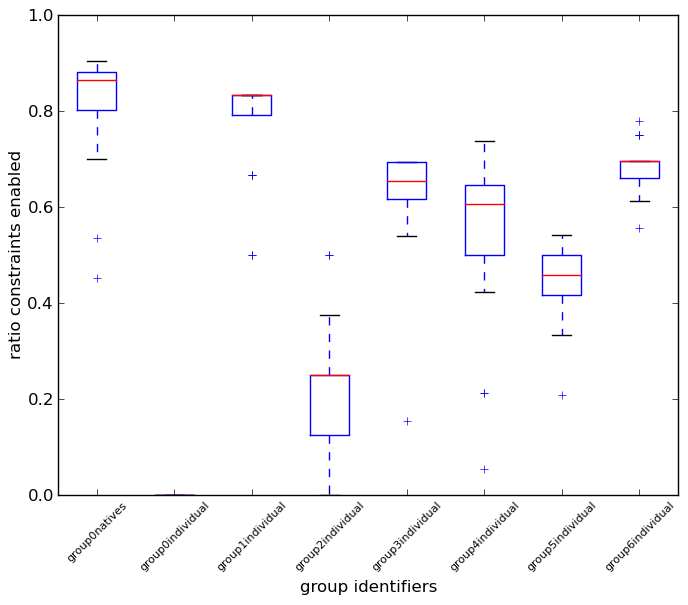
\includegraphics[width=0.7\textwidth]{enabledConstraintsIndividual.png}
    \caption{Ratio of enabled constraints for all decoys generated}
    \label{fig:enabledConstraints}
\end{figure}
    
By analyzing protein 2krkA it shows, that the highest precision is in groups 3 and 6, where the highest ratio of enabled constraints can be found in groups 1, 3 and 6.

By accounting group size, one can see that group 1 contains only 6 constraints, where group 3 contains 13 and group 6 contains 36 constraints. Clearly Rosetta has more difficulties to enable a larger number of constraints and by taking that into consideration, one can come up with a reasonable decider which group to choose best.

\section{Insights}

\begin{enumerate}
\item A high percentage of enabled constraints in a decoy also increases the percentage of native constraints in the subset.
% TODO: maybe formulate a decider, that takes the group size into account? \item The prediction accuracy does not increase with the chosen group.
\item The grouping based on secondary structure does not contain a high percentage of native constraints in every case.
\item The size of the group has an influence on the prediction quality and the percentage of enabled constraints.
\item The Rosetta energy function does not reveal any insight about the noisiness of the constraints
\end{enumerate}


\section{Future Work}

\subsection{Iterative Algorithm}

The constraint subsets could be used in an iterative algorithm,
where the grouping or the weights are modified in each iteration
and the information on fulfilled constraints after each prediction
guides the search.

\subsection{Predict non Native Constraint Subsets}

Instead of predicting native constraints and use them,
the same pipeline could be used to filter out bad constraints.
For example, in \texttt{group0individual} and \texttt{group2individual}
in Figure \ref{fig:enabledConstraints}, the ratio of enabled constraints is low,
where also the ratio of native constraints is low.
The principle would be to exclude them from further subsets.

\subsection{Adapting Weights}

In this project we used the standard weight of $1.5$ in the constraint penalty function.
But certainly, the effect of weights should be investigated in the context of
noisy constraints.

\subsection{Different Subset Generation Techniques}

The main idea of this project was subset generation based on a heuristic,
i.e. trying to exploit the information available.
The heuristic that was investigated here, was based on the type of secondary structure.
But there is a lot of other information that could have an influence on the quality
of a constraint subset, for example:
\begin{itemize}
\item distance of the residues on the sequence
\item atom and sidechain of corresponding to the constraint
\item in a second step (cf. Iterative Algorithms), group all constraints that were fulfilled or had a specific distance pattern in the decoy.
\end{itemize}
\end{document}
